\section{Diagramme des cas d'utilisation}\label{casutilisation} 

Nous avons réalisé un schéma des cas d'utilisations, visible en figure \vref{usecase} afin de synthétiser les besoins de l'utilisateur, pour offrir une vision simplifiée du système. Nous rappellerons brièvement les fonctionnalités par la suite.

\begin{figure}[h]
\begin{center}
    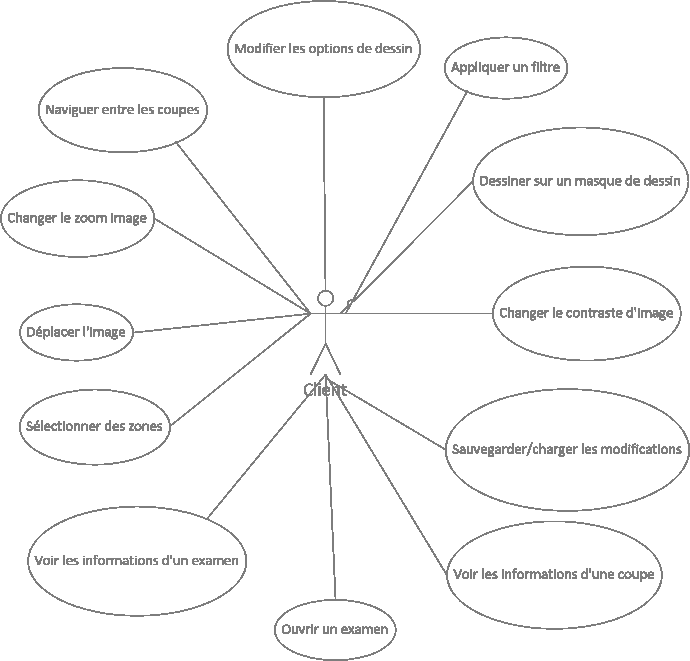
\includegraphics[width=12cm]{diagramme-usecase}
\end{center}
    \caption{Diagramme de cas d'utilisation}
    \label{usecase}                      
\end{figure}

\subsubsection{Ouvrir un examen}

L'utilisateur peut ouvrir un examen stocké sur sa tablette en parcourant l'arborescence de fichiers
et en cliquant sur l'examen choisi.

\subsubsection{Visualiser les informations d'un examen}

Le client peut, n'importe où dans un examen, visualiser les informations associées à cet examen
en cliquant sur un bouton qui déclenchera l'ouverture de la fenêtre d'affichage des informations.
Il pourra y voir des informations sur le patient et sur les conditions d'examen.

\subsubsection{Visualiser les informations d'une coupe}

Le client peut visualiser les informations associées à une coupe
en cliquant sur un bouton qui déclenchera l'ouverture de la fenêtre d'affichage des informations.
Il pourra y voir des informations associées à la coupe affichée à l'écran.

\subsubsection{Naviguer entre les coupes}

Le client peut visualiser les différentes coupes qui composent un examen qu'il a précédemment ouvert
en cliquant sur les boutons associés aux déplacements entre coupes.

\subsubsection{Dessiner des zones sur un masque de dessin}

Le client peut dessiner sur un masque de dessin en superposition avec l'image d'une coupe de l'examen.
Il dispose d'outils de dessin tels que le crayon ou la gomme.

\subsubsection{Modifier les options de dessin}

Le client peut dessiner sur un masque de dessin en variant les effets tels que l'épaisseur du trait
utilisé.

\subsubsection{Modifier le contraste de l'examen}

Le client peut à tout moment changer le contraste (échelle de Hounsfield) des coupes de l'examen ouvert
en utilisant les contrôles associés à cet effet. Il peut modifier la largeur de l'échelle et son centre.
Il peut également choisir un contraste prédéfini parmi une liste de contrastes pour visualiser des éléments
spécifiques tels que les os ou les chairs.

\subsubsection{Se déplacer dans l'image}

Le client peut visualiser différentes portions d'une image en la faisant glisser sur l'écran avec les doigts.

\subsubsection{Changer le niveau de zoom d'une image}

Le client peut modifier le niveau de zoom d'une image en utilisant le contrôle prévu à cet effet.
Il peut augmenter ou diminuer le niveau de zoom.

\subsubsection{Sauvegarder les modifications}

Le client peut enregistrer ses modifications (dessin, contraste par défaut) effectuées sur un examen.

\subsubsection{Restaurer les modifications}

Le client peut charger ses modifications (dessin, contraste par défaut) effectuées auparavant sur un examen.

\subsubsection{Appliquer un filtre}

Le client peut modifier les images d'un examen en appliquant un filtre (tel que le flou gaussien).

\subsubsection{Sélectionner des zones}

Le client peut sélectionner des zones sur une coupe pour appliquer des traitements spécifiquement sur ces
zones.